\documentclass[a4paper,10pt]{article}

%A Few Useful Packages
\usepackage{marvosym}
\usepackage{fontspec} 					%for loading fonts
\usepackage{xunicode,xltxtra,url,parskip} 	%other packages for formatting
\usepackage{graphicx}
\usepackage{lipsum}
\usepackage[export]{adjustbox}
\graphicspath{ {images/} }
\RequirePackage{color,graphicx}
\usepackage[usenames,dvipsnames]{xcolor}
\usepackage[big]{layaureo} 				%better formatting of the A4 page
% an alternative to Layaureo can be ** \usepackage{fullpage} **
\usepackage{supertabular} 				%for Grades
\usepackage{titlesec}					%custom \section

%Setup hyperref package, and colours for links
\usepackage{hyperref}
\definecolor{linkcolour}{rgb}{0,0.2,0.6}
\hypersetup{colorlinks,breaklinks,urlcolor=linkcolour, linkcolor=linkcolour}

%FONTS
\defaultfontfeatures{Mapping=tex-text}
%\setmainfont[SmallCapsFont = Fontin SmallCaps]{Fontin}
%%% modified for Karol Kozioł for ShareLaTeX use
\setmainfont[
SmallCapsFont = Fontin-SmallCaps.otf,
BoldFont = Fontin-Bold.otf,
ItalicFont = Fontin-Italic.otf
]
{Fontin.otf}
%%%

%CV Sections inspired by: 
%http://stefano.italians.nl/archives/26
\titleformat{\section}{\Large\scshape\raggedright}{}{0em}{}[\titlerule]
\titlespacing{\section}{0pt}{3pt}{3pt}
%Tweak a bit the top margin
%\addtolength{\voffset}{-1.3cm}

%Italian hyphenation for the word: ''corporations''
\hyphenation{im-pre-se}

%-------------WATERMARK TEST [**not part of a CV**]---------------
\usepackage[absolute]{textpos}

\setlength{\TPHorizModule}{30mm}
\setlength{\TPVertModule}{\TPHorizModule}
\textblockorigin{2mm}{0.65\paperheight}
\setlength{\parindent}{0pt}

%--------------------BEGIN DOCUMENT----------------------
\begin{document}

%WATERMARK TEST [**not part of a CV**]---------------
%\font\wm=''Baskerville:color=787878'' at 8pt
%\font\wmweb=''Baskerville:color=FF1493'' at 8pt
%{\wm 
%	\begin{textblock}{1}(0,0)
%		\rotatebox{-90}{\parbox{500mm}{
%			Typeset by Alessandro Plasmati with \XeTeX\  \today\ for 
%			{\wmweb \href{http://www.aleplasmati.comuv.com}{aleplasmati.comuv.com}}
%		}
%	}
%	\end{textblock}
%}

\pagestyle{empty} % non-numbered pages

\font\fb=''[cmr10]'' %for use with \LaTeX command

%--------------------TITLE-------------

\noindent
\begin{minipage}{0.7\textwidth}\centering{

		\Huge Davide \textsc{Anghileri}}
\end{minipage}
\begin{minipage}{0.3\textwidth}% adapt widths of minipages to your needs
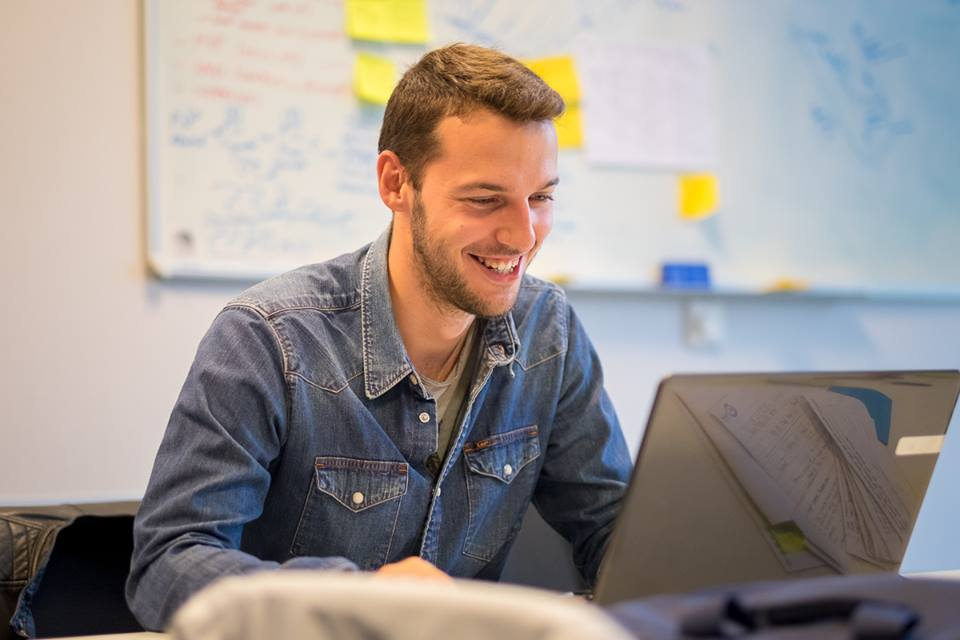
\includegraphics[trim=3cm 3cm 3cm 1cm, clip=true, scale=0.14]{Foto_Davide_EIT}\raggedright
\end{minipage}%
\hfill%



%--------------------SECTIONS-----------------------------------
%Section: Personal Data
\section{Personal Data}

\begin{tabular}{rl}
    \textsc{Place and Date of Birth:} & Lecco, Italy  | 18 August 1994 \\
    \textsc{Address:}   & Via Trebbia 75, Valmadrera (LC) 23868, Italy \\ %Osquldas  väg 18, Apt. 11119, 114 28 Stockholm
    \textsc{Phone:}     & +39 334 8911071 \\ % preferably; +46 072 7408934
    \textsc{email:}     & \href{mailto:anghileridavide@gmail.com}{anghileridavide@gmail.com}
\end{tabular}

%%%%%%%%%%%%%%%%%%%%%%%%%%%%%Section: Education%%%%%%%%%%%%%%%%%%%%%%%%%%%%%%%

\section{Education}
\begin{tabular}{r|l}

\textsc{Jul} 2018  & 
 EIT Digital Double Degree Master’s in \textsc{Data Science} \\ &
 \emph{Exit university:}  \textbf{KTH Royal Institute of Technology}, Stockholm, Grade: A \\ & 
 \emph{Entry university:} \textbf{Politecnico di Milano}, Milan, \normalsize Grade: 110/110 \\ &
\emph{Thesis:} ``\href{http://urn.kb.se/resolve?urn=urn:nbn:se:kth:diva-232059}{Using Player Modeling to Improve Automatic Playtesting}'' \\ & Supervisor at KTH: Pawel \textsc{Herman}, Supervisor at Polimi: Pier Luca \textsc{Lanzi},\\ & Supervisor at King: Stefan Freyr \textsc{Gudmundsson} \\
 
\multicolumn{2}{c}{}\\
 
\textsc{Aug} 2017 & 
Wellbeing Summer School at \textbf{High Tech Campus}, Eindhoven \\ &
Focus on Entrepreneurial behavior, Start-ups, Pitching and Team working \\ 

\multicolumn{2}{c}{}\\

\textsc{July} 2016 & 
Bachelor of Science in \textsc{Engineering of Computing Systems} \\ &
Grade 110/110, \normalsize\textbf{Politecnico di Milano}, Milan \\ &
Final Examination: ``Software Engineering Project'' | Examiner: Marco \textsc{Brambilla} \\

%REMOVED &\\ \textsc{July} 2013& High school institute \textbf{“G. Parini”}, Lecco | Accountant
\end{tabular}

%%%%%%%%%%%%%%%%%%%%Section: Work Experience at the top%%%%%%%%%%%%%%%%%%%%%%%%%

\section{Work Experience}
\begin{tabular}{r|p{11cm}}

\textsc{2018} &
Master Thesis Intern at King, \emph{Data Science} \\ &
\textbf{King Digital Entertainment Ltd}, Sveavägen 44, 11134 Stockholm, Sweden \\ &
\small{Worked on my thesis project about Player Modeling and Automatic Playtesting in the AI R\&D team. Improved the automatic level difficulty estimation process.} \\ 

\multicolumn{2}{c}{}\\

\textsc{Summer 2012} &
Summer Internship at Bank \textsc{Popolare di Sondrio}, \emph{Finance} \\ &
\textbf{Popolare di Sondrio}, Corso Martiri della Liberazione 65, 23900 LC, Italy \\ &
\small{Worked with the finance team in portfolio management, helped with accountant receivable and payable, supported the payment team in daily operations.}\\

\multicolumn{2}{c}{}\\
 
\textsc{Feb 2012} &
Intern at a Business Consultant Firm, \emph{Accountant} \\ &
\textbf{Dr. Rocca Antonio}, Piazza Affari 12, 23900 LC, Italy \\ &
\small{Customer service regarding bills and account keeping. Increased the company’s efficiency by archiving documents and sale bills and preparing letters.} \\

\multicolumn{2}{c}{}\\
 
\textsc{Feb 2011} &
Intern at a Chartered Accountants Firm, \emph{Accountant} \\ &
\textbf{So.Ge.Co. S.a.s. di Pecis Pietro e C.}, Corso Martiri 112, 23900 LC, Italy \\ &
\small{Customer relationship, kept billings, accounts and inserted purchases.} \\ 

\multicolumn{2}{c}{}\\
\end{tabular}


%%%%%%%%%%%%%%%%%%%%Certificates, Workshops and Projects%%%%%%%%%%%%%%%%%%%%%%%%
\section{Certificates, Workshops and Projects}
\begin{tabular}{r|p{12cm}}

\textsc{Spring} 2018 &
\href{https://drive.google.com/file/d/1b_lHlvgywHEauQFdMg_j-ndgBh4n7KJT/view?usp=sharing}{\textsc{Minor Thesis Project within Entrepreneurship}} \newline \small{Title: Ethics and Implications of the Free-to-Play Business Model in the Game Industry} \\

\multicolumn{2}{c}{}\\

\textsc{Dec} 2017 &
\href{https://drive.google.com/file/d/1Ek7kZRvnRRklJAh8rlvWSrI8kMXpoxS4/view?usp=sharing}{\textsc{Research Methodology and Scientific Writing Project}} \newline \small{Title: Exploratory Study of Island-Based Parallel Differential Evolution Algorithms using Apache Spark} \\

\multicolumn{2}{c}{}\\

\textsc{Sept} 2017 &
\href{https://www.researchgate.net/publication/318542744_Enhancing_Children's_Experience_with_Recommendation_Systems}{\textsc{Enhancing Children’s Experience with Recommendation Systems}} \newline \small{\emph{Davide Anghileri, Y. Deldjoo, C. Fra, M. Valla, A. Paladini, M.A. Tuncil, F. Garzotta, P. Cremonesi,}} Proceedings of the 11th ACM Conference of Recommender Systems, 2017. \\

\multicolumn{2}{c}{}\\

\textsc{Jun} 2017 &
\href{https://www.youtube.com/watch?v=AbMl5wnMQrg&t=4s}{\textsc{Mise-en-Scène}} \newline \small{A movie recommender Web-App in collaboration with Telecom Italia Joint Open Lab (JOL) in Milan, to study the influence of personality traits in recommendations and to create an interactive DVD cover recognizer to automatically build a user profile.}  \\

\multicolumn{2}{c}{}\\

\textsc{May} 2017 &
\href{https://www.kaggle.com/c/recommender-system-2016-challenge-polimi/leaderboard}{\textsc{Kaggle competition in recommender systems}}  \\

\multicolumn{2}{c}{}\\

\textsc{Spring} 2017 &
\href{https://www.youtube.com/watch?v=3uLLvG1s0R0}{\textsc{Digital Business Innovation Lab Project}} \newline
\small{A Web-App that thanks to IBM Watson technology can understand the user style from his/her photos on social networks and recommend new fashionable outfits.} \\ 

\multicolumn{2}{c}{}\\

\textsc{March} 2016 & LabView certified associate Developer.\\

\end{tabular}

\section{Languages}
\textsc{Mother tongue:} Italian, \\ \textsc{Others:} English (\emph{C1 - TOEIC certification with a score of 815}), Spanish (\emph{A2}) 

\section{Programming skills}
I have competences in Python, C, C++, Java, SQL, HTML, CSS and JavaScript and basic knowledge of React, MongoDB and others.

\section{Communication skills}

Technical and scientific writing skills gained at KTH university. \\
Divergent thinking and brainstorming skills gained through my summer school in Eindhoven. \newline Marketing, visualization and presentation skills gained during Strategy and Marketing courses.

\section{Organisational skills}

Collaboration and teamwork skills gained through my experience as a football player. \newline
Management and planning skills gained during my High school studies.

\section{Interests and Activities}
Technology, Entrepreneurship, Big-Data, Start-Ups, AI, Machine Learning and Logic.\\
Football, Running and Travelling.



\end{document}
